%%%%%%%%%%%%%%%%%%%%%%%%%%%%%%%%%%%%%%%%%%%%%%%%%%%%%%%%%%%%%%%%%%%%%
%%                                                                 %%
%% Please do not use \input{...} to include other tex files.       %%
%% Submit your LaTeX manuscript as one .tex document.              %%
%%                                                                 %%
%% All additional figures and files should be attached             %%
%% separately and not embedded in the \TeX\ document itself.       %%
%%                                                                 %%
%%%%%%%%%%%%%%%%%%%%%%%%%%%%%%%%%%%%%%%%%%%%%%%%%%%%%%%%%%%%%%%%%%%%%

%%\documentclass[referee,sn-basic]{sn-jnl}% referee option is meant for double line spacing

%%=======================================================%%
%% to print line numbers in the margin use lineno option %%
%%=======================================================%%

%%\documentclass[lineno,sn-basic]{sn-jnl}% Basic Springer Nature Reference Style/Chemistry Reference Style

%%======================================================%%
%% to compile with pdflatex/xelatex use pdflatex option %%
%%======================================================%%

%%\documentclass[pdflatex,sn-basic]{sn-jnl}% Basic Springer Nature Reference Style/Chemistry Reference Style

%%\documentclass[sn-basic]{sn-jnl}% Basic Springer Nature Reference Style/Chemistry Reference Style
\documentclass[sn-mathphys]{sn-jnl}% Math and Physical Sciences Reference Style
%%\documentclass[sn-aps]{sn-jnl}% American Physical Society (APS) Reference Style
%%\documentclass[sn-vancouver]{sn-jnl}% Vancouver Reference Style
%%\documentclass[sn-apa]{sn-jnl}% APA Reference Style
%%\documentclass[sn-chicago]{sn-jnl}% Chicago-based Humanities Reference Style
%%\documentclass[sn-standardnature]{sn-jnl}% Standard Nature Portfolio Reference Style
%%\documentclass[default]{sn-jnl}% Default
%%\documentclass[default,iicol]{sn-jnl}% Default with double column layout

%%%% Standard Packages
%%<additional latex packages if required can be included here>
%%%%

%%%%%=============================================================================%%%%
%%%%  Remarks: This template is provided to aid authors with the preparation
%%%%  of original research articles intended for submission to journals published 
%%%%  by Springer Nature. The guidance has been prepared in partnership with 
%%%%  production teams to conform to Springer Nature technical requirements. 
%%%%  Editorial and presentation requirements differ among journal portfolios and 
%%%%  research disciplines. You may find sections in this template are irrelevant 
%%%%  to your work and are empowered to omit any such section if allowed by the 
%%%%  journal you intend to submit to. The submission guidelines and policies 
%%%%  of the journal take precedence. A detailed User Manual is available in the 
%%%%  template package for technical guidance.
%%%%%=============================================================================%%%%

\jyear{2021}%

%% as per the requirement new theorem styles can be included as shown below
\theoremstyle{thmstyleone}%
\newtheorem{theorem}{Theorem}%  meant for continuous numbers
%%\newtheorem{theorem}{Theorem}[section]% meant for sectionwise numbers
%% optional argument [theorem] produces theorem numbering sequence instead of independent numbers for Proposition
\newtheorem{proposition}[theorem]{Proposition}% 
%%\newtheorem{proposition}{Proposition}% to get separate numbers for theorem and proposition etc.

\theoremstyle{thmstyletwo}%
\newtheorem{example}{Example}%
\newtheorem{remark}{Remark}%

\theoremstyle{thmstylethree}%
\newtheorem{definition}{Definition}%

\raggedbottom
%%\unnumbered% uncomment this for unnumbered level heads

% Landscape pages for tables
\usepackage{lscape}


\begin{document}

\title[Innovation and elaboration on the avian tree of life]{Innovation and elaboration on the avian tree of life - supplementary materials}

%%=============================================================%%
%% Prefix   -> \pfx{Dr}
%% GivenName    -> \fnm{Joergen W.}
%% Particle -> \spfx{van der} -> surname prefix
%% FamilyName   -> \sur{Ploeg}
%% Suffix   -> \sfx{IV}
%% NatureName   -> \tanm{Poet Laureate} -> Title after name
%% Degrees  -> \dgr{MSc, PhD}
%% \author*[1,2]{\pfx{Dr} \fnm{Joergen W.} \spfx{van der} \sur{Ploeg} \sfx{IV} \tanm{Poet Laureate} 
%%                 \dgr{MSc, PhD}}\email{iauthor@gmail.com}
%%=============================================================%%

\author*[1]{\fnm{Thomas} \sur{Guillerme}}\email{guillert@tcd.ie}

\author[2]{\fnm{Natalie} \sur{Cooper}}\email{natalie.cooper@nhm.ac.uk}

\author[1]{\fnm{Andrew P.} \sur{Beckerman}}\email{a.beckerman@sheffield.ac.uk}

\author[1]{\fnm{Gavin H.} \sur{Thomas}}\email{gavin.thomas@sheffield.ac.uk}

\affil*[1]{\orgdiv{School of Biosciences}, \orgname{University of Sheffield}, \orgaddress{\city{Sheffield}, \postcode{S10 2TN}, \country{UK}}}

\affil[2]{\orgname{Natural History Museum}, \orgaddress{\street{Cromwell Road}, \city{London}, \postcode{SW75BD}, \country{UK}}}

%%==================================%%
%% sample for unstructured abstract %%
%%==================================%%

\abstract{The abstract serves both as a general introduction to the topic and as a brief, non-technical summary of the main results and their implications. Authors are advised to check the author instructions for the journal they are submitting to for word limits and if structural elements like subheadings, citations, or equations are permitted.}

%%================================%%
%% Sample for structured abstract %%
%%================================%%

% \abstract{\textbf{Purpose:} The abstract serves both as a general introduction to the topic and as a brief, non-technical summary of the main results and their implications. The abstract must not include subheadings (unless expressly permitted in the journal's Instructions to Authors), equations or citations. As a guide the abstract should not exceed 200 words. Most journals do not set a hard limit however authors are advised to check the author instructions for the journal they are submitting to.
% 
% \textbf{Methods:} The abstract serves both as a general introduction to the topic and as a brief, non-technical summary of the main results and their implications. The abstract must not include subheadings (unless expressly permitted in the journal's Instructions to Authors), equations or citations. As a guide the abstract should not exceed 200 words. Most journals do not set a hard limit however authors are advised to check the author instructions for the journal they are submitting to.
% 
% \textbf{Results:} The abstract serves both as a general introduction to the topic and as a brief, non-technical summary of the main results and their implications. The abstract must not include subheadings (unless expressly permitted in the journal's Instructions to Authors), equations or citations. As a guide the abstract should not exceed 200 words. Most journals do not set a hard limit however authors are advised to check the author instructions for the journal they are submitting to.
% 
% \textbf{Conclusion:} The abstract serves both as a general introduction to the topic and as a brief, non-technical summary of the main results and their implications. The abstract must not include subheadings (unless expressly permitted in the journal's Instructions to Authors), equations or citations. As a guide the abstract should not exceed 200 words. Most journals do not set a hard limit however authors are advised to check the author instructions for the journal they are submitting to.}

\keywords{keyword1, Keyword2, Keyword3, Keyword4}


\maketitle

\section{Supplementary material 1}

\begin{figure}[!htbp]
\centering
   \includegraphics[width=0.9\textwidth]{Figures/figure_cheat_sheet.pdf}
\caption{Relation between the figures in the main text.
The top left panel represents the two first dimensions of the 8 dimensional trait space with all bird beaks represented as grey circles and the Palaeognathes as red ones.
The grey ellipse represents the average posterior variance covariance matrix (VCV) from the general phylogenetic random term of the MCMCglmm model (i.e. the overall phylogenetic axis of main variation).
Species aligned with this axis tend to be elaborators at the mega-evolutionary level and species going away from that line are innovators at the mega-evolutionary level.
The red ellipse and axis represents the average posterior VCV for the Palaeognathes only.
Species position on this axis elaborate and innovate at the macro-evolutionary level.
On the top right panel (Figure 1 in the main text), we measured the elaboration and innovation at the entire clade level (cf. at the species level below).
The ellipses are a scaled and centered in space representation of the group’s VCV ellipse relative to the overall phylogenetic one with a the relative length of the ellipse on each dimension represented on the barplots.
The clade's innovation and elaboration scores are measured by projecting the clade's major axis onto the phylogenetic one and measuring the projection (elaboration) and rejection (innovation) as mentioned above.
The distribution of innovation and elaboration scores comes from the projection of the 4000 pairs of posterior VCVs.
On the bottom right panel (Figure 3 in the main text), we measured the position of each species in terms of elaboration and innovation.
A species elaboration score is their projection onto the phylogenetics' VCV major axis (i.e. their position on that axis) whereas their innovation score is their rejection from it (i.e. their distance away from that axis).}
\label{Fig:cheat_sheet}
\end{figure}


\begin{figure}[!htbp]
\centering
   \includegraphics[width=0.9\textwidth]{Figures/Supplementary_figure_axis_selection.pdf}
\caption{variance and cumulative variance for each 8 axis per super-order.}
\label{Fig:axes_variance}
\end{figure}


\begin{figure}[!htbp]
\centering
   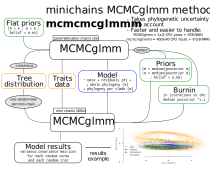
\includegraphics[width=0.9\textwidth]{Figures/mini-chains_diagram.pdf}
\caption{mcmcmcglmmm: mini-chains MCMCglmm method diagram}
\label{Fig:fig_mcmcmcglmm}
\end{figure}


\begin{figure}[!htbp]
\centering
   \includegraphics[width=0.5\textwidth]{Figures/parameters_ESS_all_birds.pdf}
\caption{Histogram of the effective sample sizes (ESS) for each class of parameters in the MCMCglmm model for all birds for the 4000 posteriors. \textbf{solution} is the solution of the model; \textbf{Gcovariance} are the covariances for the random terms (the phylogeny and the clades); \textbf{Rcovariance} are the residuals error term.}
\label{Fig:model_ess_all_birds}
\end{figure}

\begin{figure}[!htbp]
\centering
   \includegraphics[width=0.5\textwidth]{Figures/parameters_ESS_passeriformes.pdf}
\caption{Histogram of the effective sample sizes (ESS) for each class of parameters in the MCMCglmm model for the passeriformes for the 1870 posteriors. \textbf{solution} is the solution of the model; \textbf{Gcovariance} are the covariances for the random terms (the phylogeny and the clades); \textbf{Rcovariance} are the residuals error term.}
\label{Fig:model_ess_passeriformes}
\end{figure}

%TODO:TG: update the passeriformes parameters estimate (with more models)

\begin{landscape}
\input{Tables/Tab_variance_per_axis.tex}
\end{landscape}

\section{Supplementary material 2: Passeriformes results}



\begin{figure}[!htbp]
\centering
   \includegraphics[width=0.9\textwidth]{Figures/Supplementary_figure_axis_selection.pdf}
\caption{variance and cumulative variance for each 8 axis per super-order.}
\label{fig_ellipses_passeriformes}
\end{figure}


Figure {#fig_ellipses}: elaboration and innovation at the group level. Panel A) shows  ellipses representing the scaled median posterior variance-covariance response from the pGLMM models for each superorder (coloured ellipses) compared to the all-birds phylogenetic component of the models (grey ellipses). We scaled the ellipses so the length of the major axis of the clade ellipses is the same length as that of the global ellipse (in eight dimensions). The first inset ellipse plot shows the positions of all superorder ellipses relative to the all-bird phylogenetic ellipse. Subsequent inset plots show the results for each superorder. Inset barplots show the proportion of variance associated with each of the eight PC axes in shape morphospace.. The inset boxplots correspond to the elaboration (E) and innovation (I) scores  for all 4000 posterior samples. The dots represent the median elaboration and innovation values while the thick and dashed lines represent the 50% and 95% confidence intervals respectively. Note that these scores were calculated on the unscaled ellipses resulting in different scales of elaboration and innovation scores for each plot. Panel B) shows  the results for each order.

Figure {#fig_orthogonality}. Posterior results showing the orientation of phenotypic evolution (orthogonality)of each group compared to their parent clade or to their parent’s parent clade. Orthogonality scales from 0 (modulo of 0°) to 1 (modulo of 90°). For each clade we indicate the number of species (n) and the standard deviation of ellipse orientation within the clade (sd; expressed in degrees). The lines represent the 95% credibility interval of the 4000 variance-covariance ellipses and the dots represent their median orthogonality value. Opaque lines represent the comparisons between the group’s ellipse and their parent clade and semi-transparent lines represent their comparison to their parent’s parent clade. The background grey and dashed grey lines represent respectively an orthogonality of 0.5 (modulo of 45°) and 0.75 (modulo of 67.5°) Note that some clades are both similarly orthogonal to their parent and parent’s parent clade (e.g. Pterocliformes) while some are not (e.g. Columbiformes). 

The avian phylogeny (n = 8748 species) coloured by speciesbeak shape innovation and elaboration level. Blue and yellow colors highlight species with relatively low elaboration or low innovation, whereas orange to red colours indicate high innovation or elaboration. Innovations and elaboration are displayed as: a)comparisons of species to the phylogenetic major axis (inner two bands); b) comparisons of species to their superorder major axis (middle two bands); and c) comparisons of species to their order major axis (outer two bands). The branches are coloured by the species distance from the centroid of the shapespace and the estimation of their ancestors’ position in that space. A companion plot showing further nested structure within the Passeriformes is shown in Fig {supplementary_figure_passerines}.


\bibliography{sn-bibliography}% common bib file
%% if required, the content of .bbl file can be included here once bbl is generated
%%\input sn-article.bbl

%% Default %%
%%\input sn-sample-bib.tex%

\end{document}
